\documentclass{article}
\usepackage{xcolor}
\usepackage{titleps}
\usepackage[letterpaper, margin=0.95in]{geometry}
\usepackage{url}
\usepackage{amsmath}
\usepackage{amssymb}
\usepackage{wrapfig}
\usepackage{float}
\usepackage{mathtools}
\usepackage{enumitem}
\usepackage{tabu}
\usepackage{parskip}
\usepackage{natbib}
\usepackage{listings}
\usepackage{tikz}
\usepackage{quiver}
\usepackage{graphicx}

\newcommand{\xb}{\mathbf{x}}
\newcommand{\yb}{\mathbf{y}}
\newcommand{\wb}{\mathbf{w}}
\newcommand{\Xb}{\mathbf{X}}
\newcommand{\Yb}{\mathbf{Y}}
\newcommand{\tr}{^T}
\newcommand{\hb}{\mathbf{h}}
\newcommand{\Hb}{\mathbf{H}}

\DeclareFontShape{OT1}{cmtt}{bx}{n}{<5><6><7><8><9><10><10.95><12><14.4><17.28><20.74><24.88>cmttb10}{}


\usepackage{forest}

\usepackage{hyperref}
\usepackage[color=red]{todonotes}
\usepackage{forest}
\definecolor{light-yellow}{HTML}{FFE5CC}

\usepackage{cleveref}

\newpagestyle{ruled}
{\sethead{Berkeley CS 285}{Deep Reinforcement Learning, Decision Making, and Control}{Fall 2023}\headrule
  \setfoot{}{}{}}
\pagestyle{ruled}

\renewcommand\makeheadrule{\color{black}\rule[-.75\baselineskip]{\linewidth}{0.4pt}}
\renewcommand*\footnoterule{}

\begin{document}
\lstset{basicstyle = \ttfamily,columns=fullflexible,
backgroundcolor = \color{light-yellow}
}

\begin{centering}
    {\Large Assignment 4: Model-Based RL} \\
    \vspace{.25cm}
    \textbf{Due December 3rd, 11:59 pm} \\
\end{centering}

\section*{Problem 1}
\begin{figure}[htbp]
    \centering
    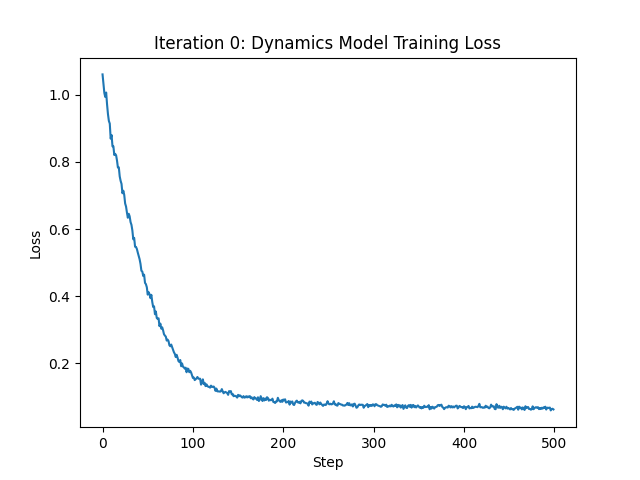
\includegraphics[width=0.8\textwidth]{p1_original_loss_curve.png}
    \caption{Learning curve for original run}
\end{figure}

\begin{figure}[htbp]
    \centering
    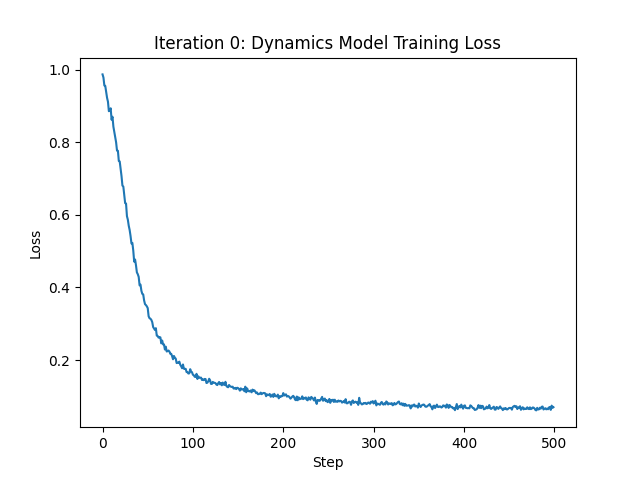
\includegraphics[width=0.8\textwidth]{p1_layer3_loss_curve.png}
    \caption{Learning curve for a 3-layer network}
\end{figure}

\begin{figure}[htbp]
    \centering
    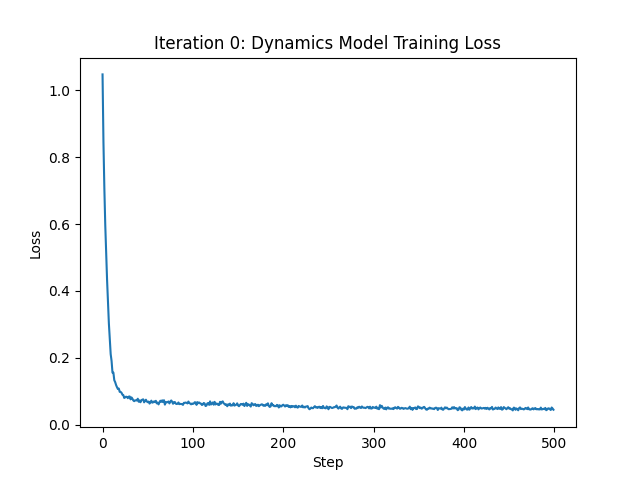
\includegraphics[width=0.8\textwidth]{p1_lr0.01_loss_curve.png}
    \caption{Learning curve for learning rate = 0.01}
\end{figure}

\newpage
\section*{Problem 2}
\begin{figure}[htbp]
    \centering
    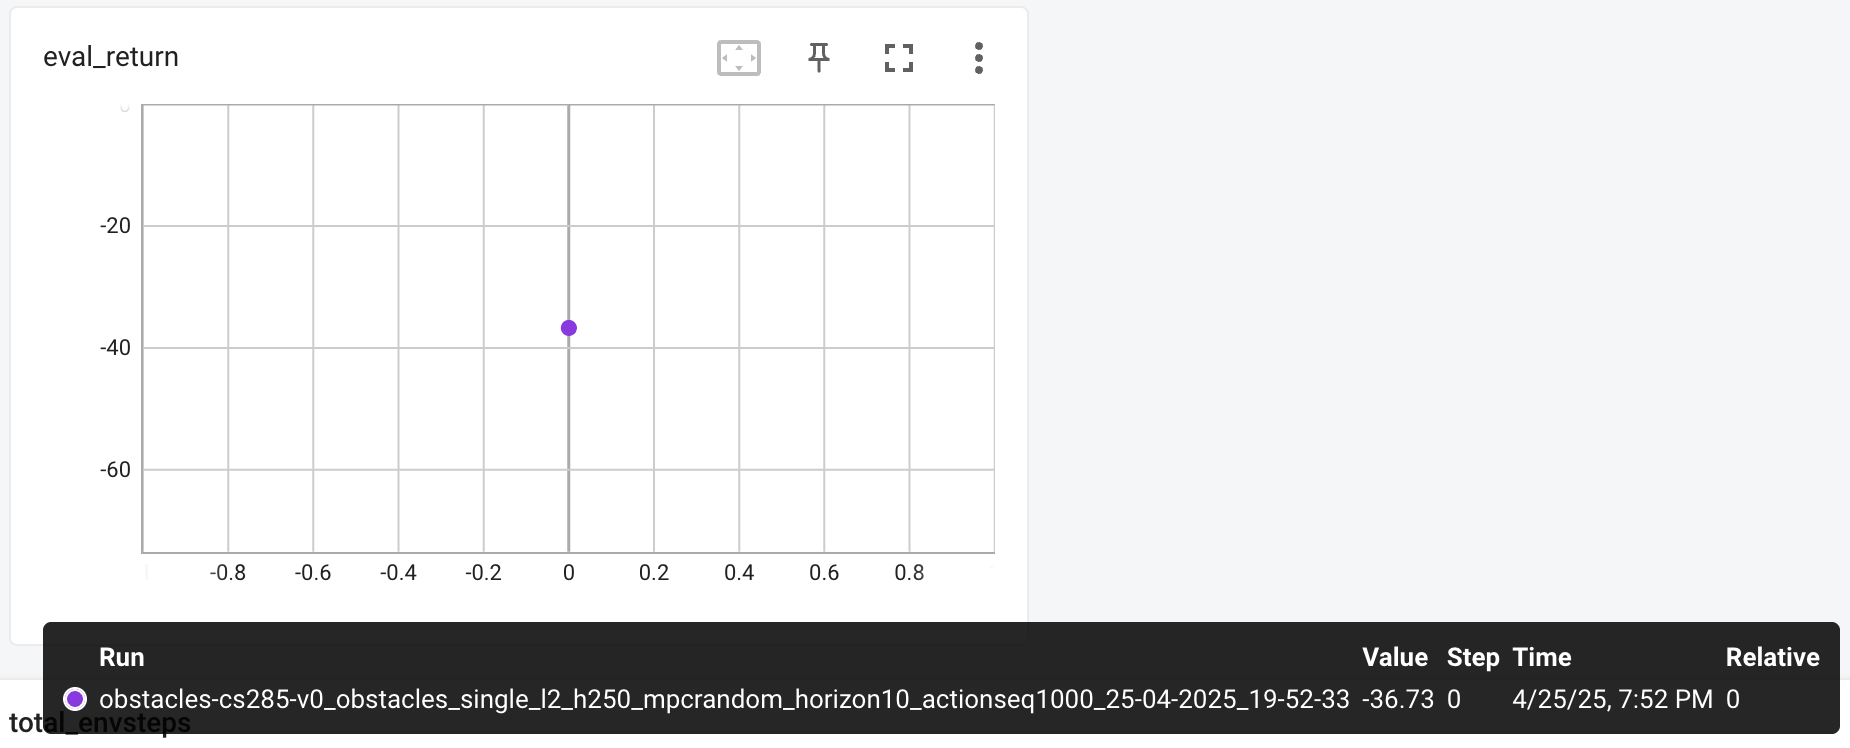
\includegraphics[width=0.8\textwidth]{p2_eval_return.png}
    \caption{Eval return achieved: -36.73}
\end{figure}

\newpage
\section*{Problem 3}
\begin{figure}[htbp]
    \centering
    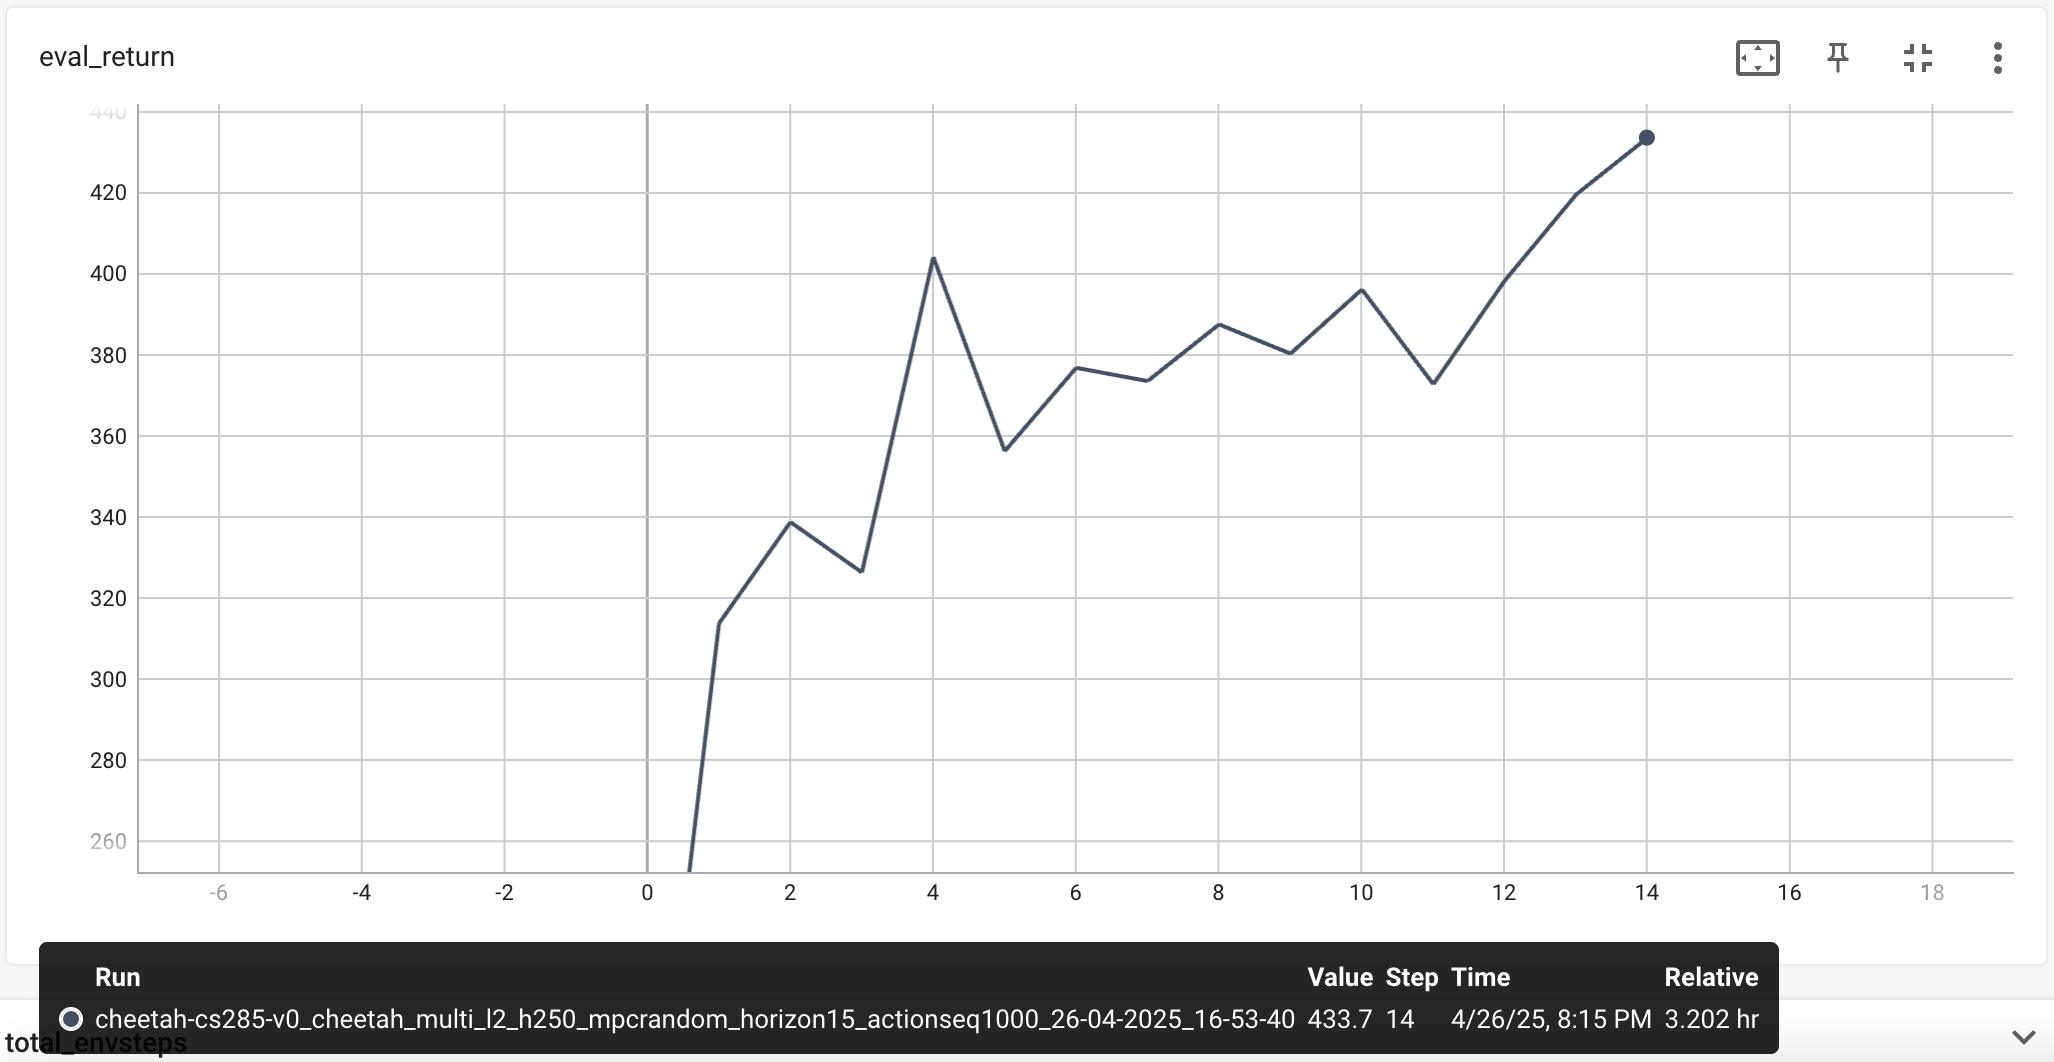
\includegraphics[width=0.8\textwidth]{p3_cheetah_eval_return.png}
    \caption{Eval return for Cheetah}
\end{figure}
\begin{figure}[htbp]
    \centering
    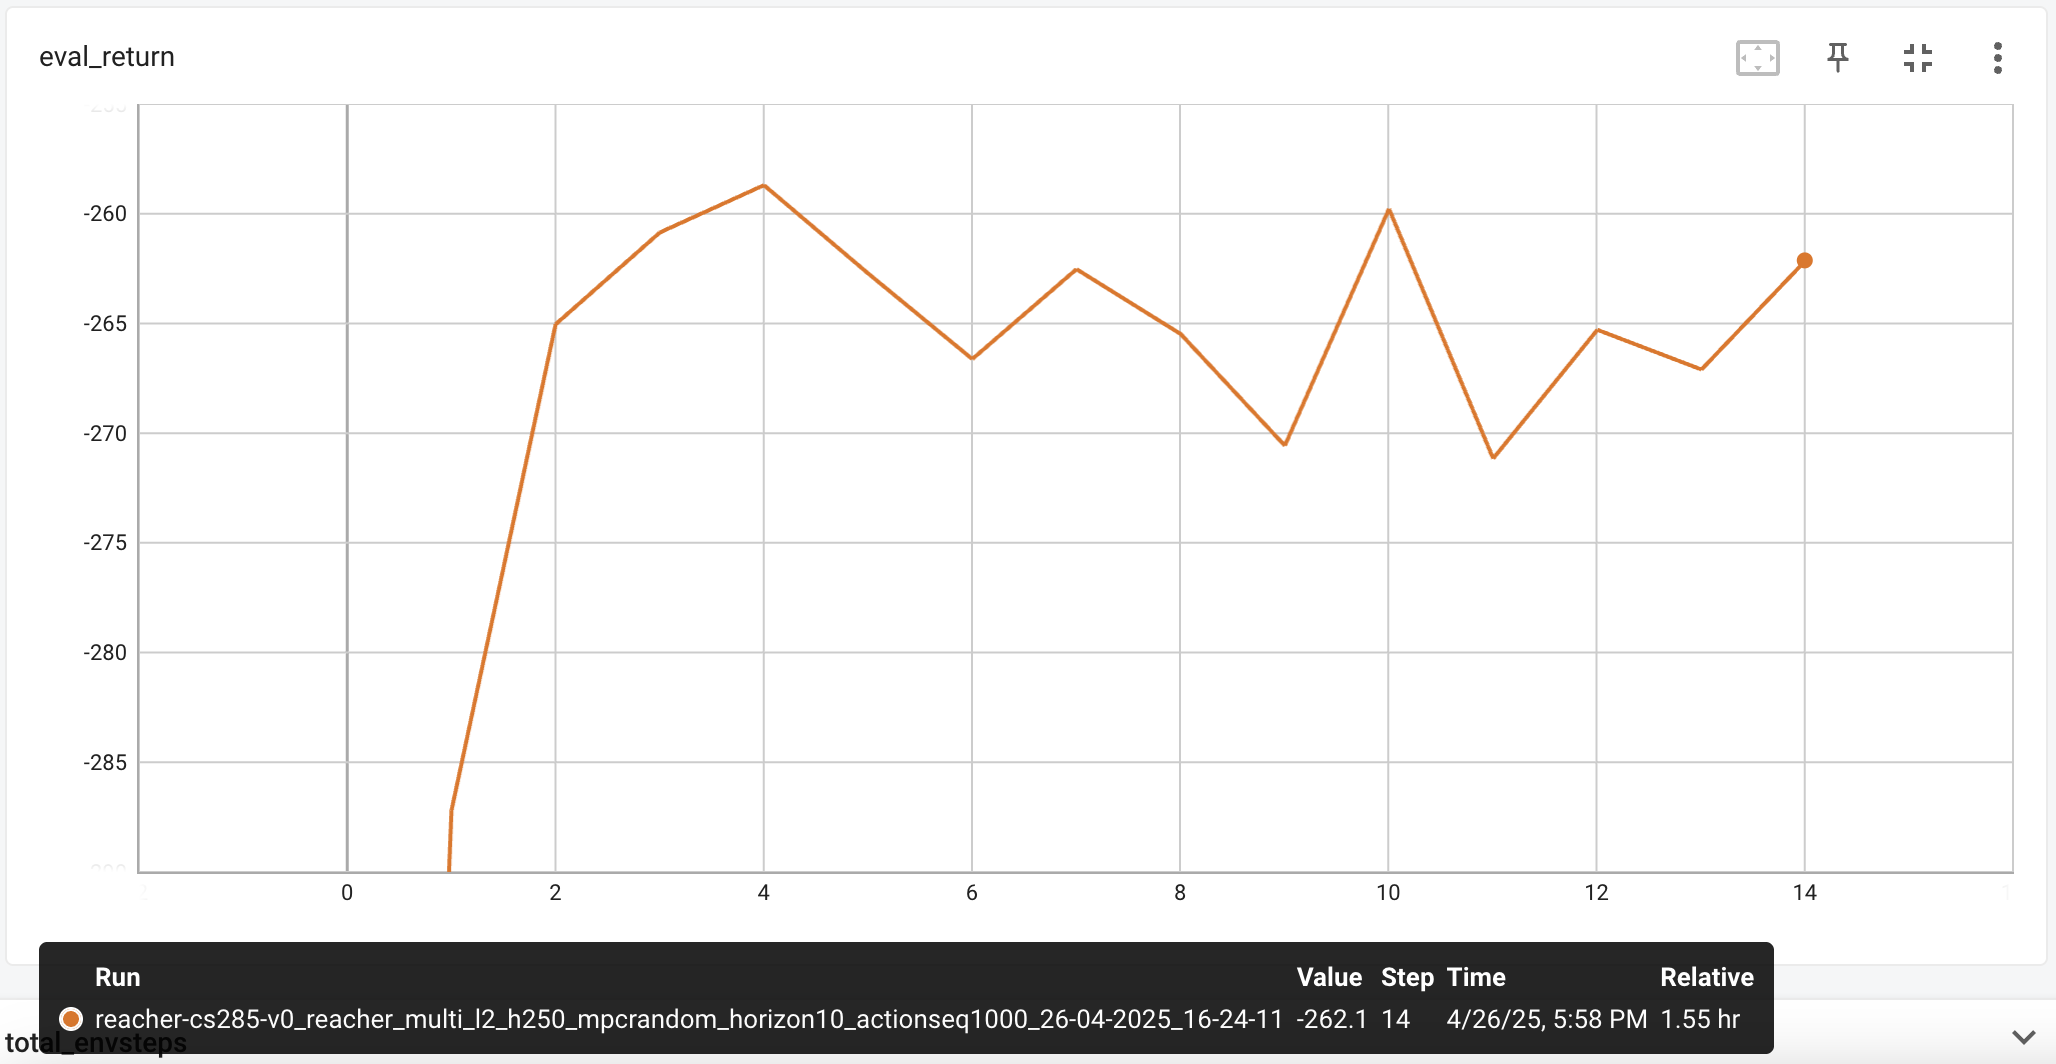
\includegraphics[width=0.8\textwidth]{p3_reacher_eval_return.png}
    \caption{Eval return for Reacher}
\end{figure}
\begin{figure}[htbp]
    \centering
    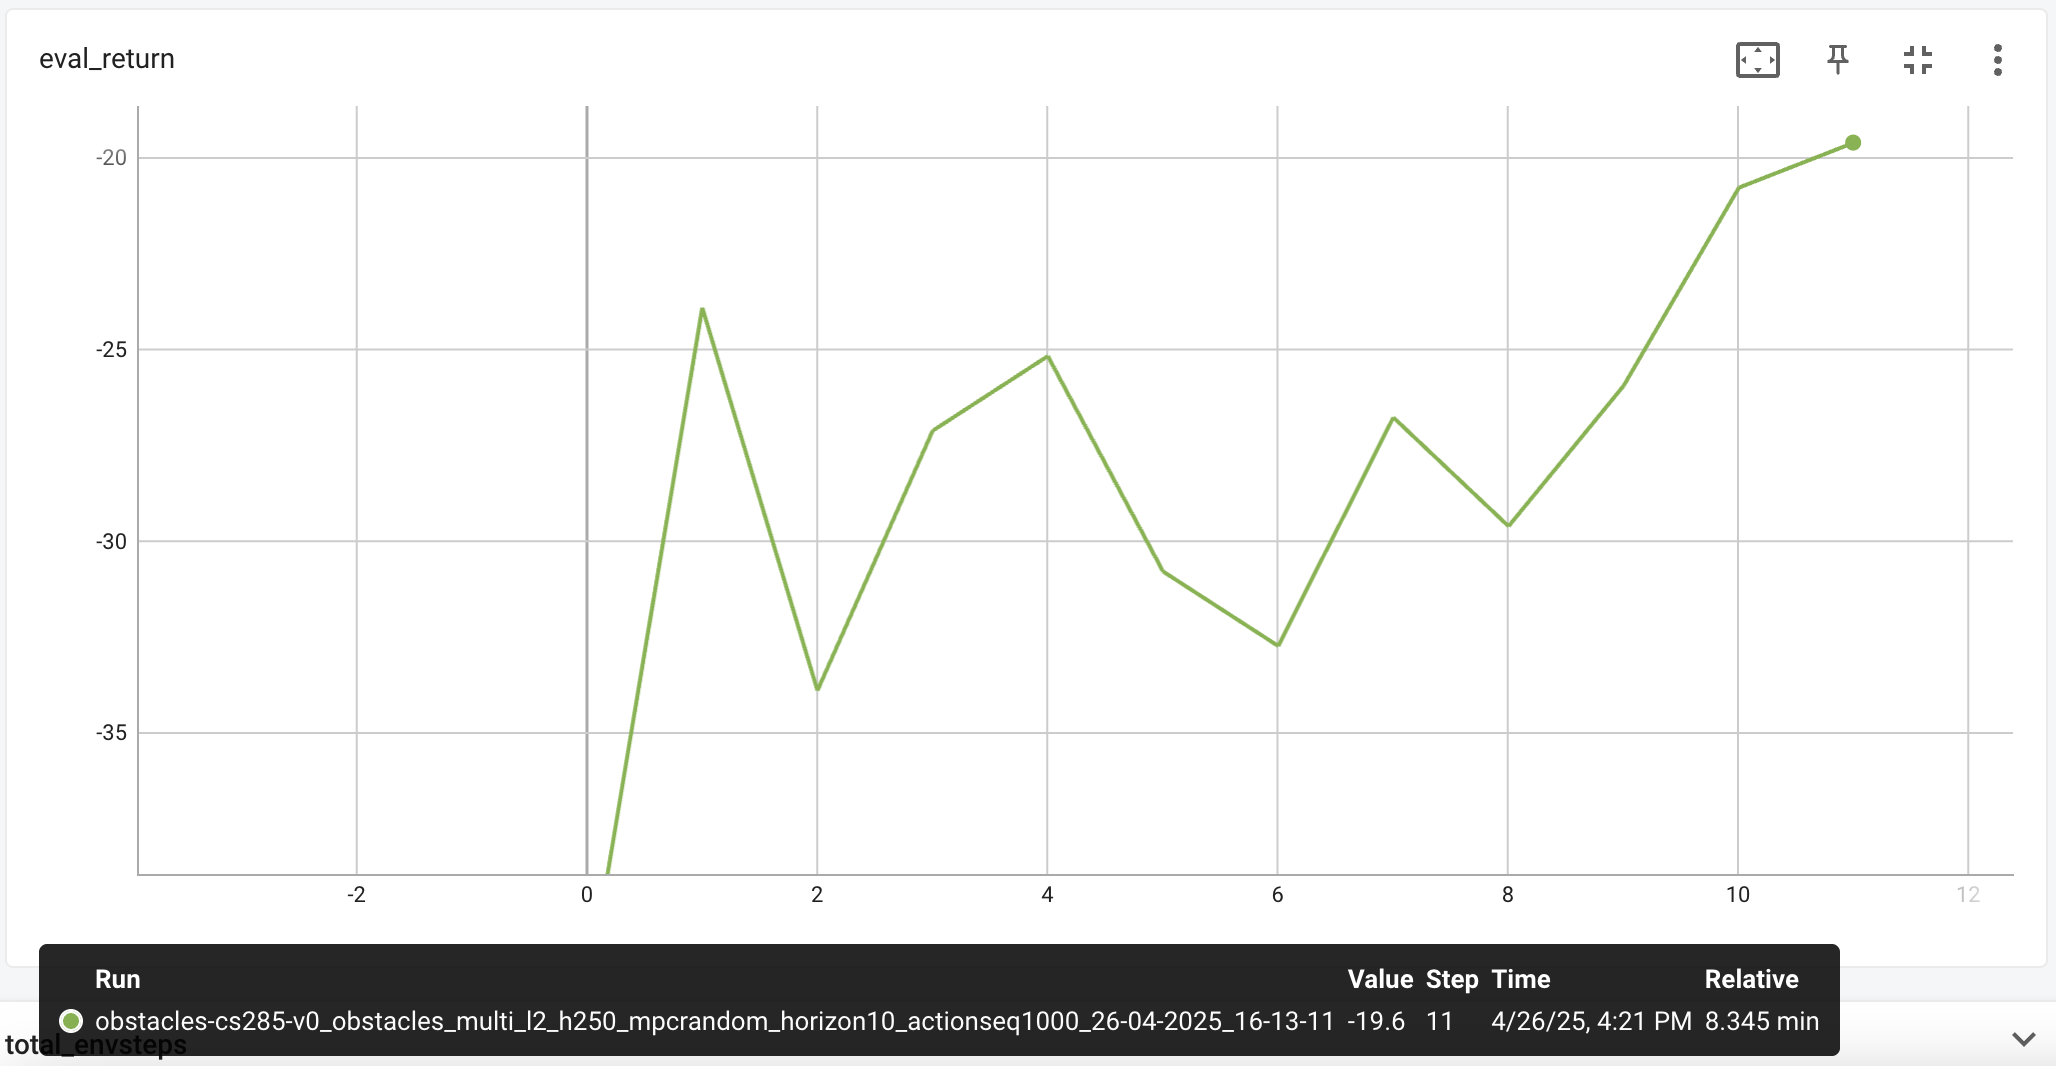
\includegraphics[width=0.8\textwidth]{p3_obstacles_eval_return.png}
    \caption{Eval return for Obstacles}
\end{figure}

\end{document}
